\documentclass[10pt]{article}
\usepackage[T1]{fontenc}
\usepackage{lmodern}
\usepackage{mathtools}
\usepackage{booktabs}
\usepackage{adjustbox}
\usepackage[left=1.5cm, right=2cm, top=1.5cm, bottom=2cm]{geometry}
\usepackage{tikz}
\usepackage{pgfplots}
\pgfplotsset{compat=1.18}
\usetikzlibrary{arrows.meta,positioning,calc}
\setlength\parindent{0pt}
\title{g7 4 - No Protection - Custom Algorithm - Descending}
\date{}
\author{}

\begin{document}
\maketitle
\section*{Topology}
\begin{center}\begin{adjustbox}{max width=\linewidth}
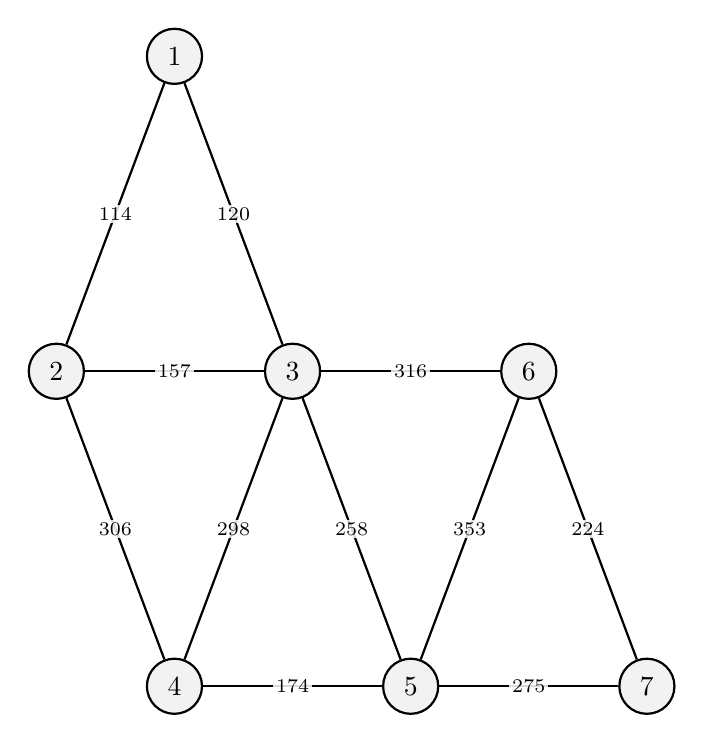
\begin{tikzpicture}[baseline, >={Stealth[length=2mm]},
  netnode/.style={circle, draw, thick, fill=gray!10, minimum size=7mm, inner sep=1pt},
  link/.style={thick},
  linklabel/.style={font=\scriptsize, inner sep=1pt, fill=white, fill opacity=0.85, text opacity=1}]
\node[netnode] (S1) at (1.500,8.000) {1};
\node[netnode] (S2) at (0.000,4.000) {2};
\node[netnode] (S3) at (3.000,4.000) {3};
\node[netnode] (S4) at (1.500,0.000) {4};
\node[netnode] (S5) at (4.500,0.000) {5};
\node[netnode] (S6) at (6.000,4.000) {6};
\node[netnode] (S7) at (7.500,0.000) {7};
\draw[link] (S1) to node[linklabel] {114} (S2);
\draw[link] (S1) to node[linklabel] {120} (S3);
\draw[link] (S2) to node[linklabel] {157} (S3);
\draw[link] (S2) to node[linklabel] {306} (S4);
\draw[link] (S3) to node[linklabel] {298} (S4);
\draw[link] (S3) to node[linklabel] {258} (S5);
\draw[link] (S3) to node[linklabel] {316} (S6);
\draw[link] (S4) to node[linklabel] {174} (S5);
\draw[link] (S5) to node[linklabel] {353} (S6);
\draw[link] (S5) to node[linklabel] {275} (S7);
\draw[link] (S6) to node[linklabel] {224} (S7);
\end{tikzpicture}
\end{adjustbox}\end{center}
\section*{Performance Parameters}
\begin{center}\begin{tabular}{lr}
\toprule
Highest link load & 582 Gb/s \\
Highest used FSU & 127 / 320 \\
Total used FSUs & 126 \\
Transponder cost & 81.5 \\
\midrule
SC-DP-QPSK transponders & 5 \\
SC-DP-16QAM transponders & 37 \\
DP-16QAM transponders & 0 \\
\bottomrule
\end{tabular}\end{center}
\clearpage
\section*{Link Load Map}
\begin{center}\begin{adjustbox}{max width=\linewidth}
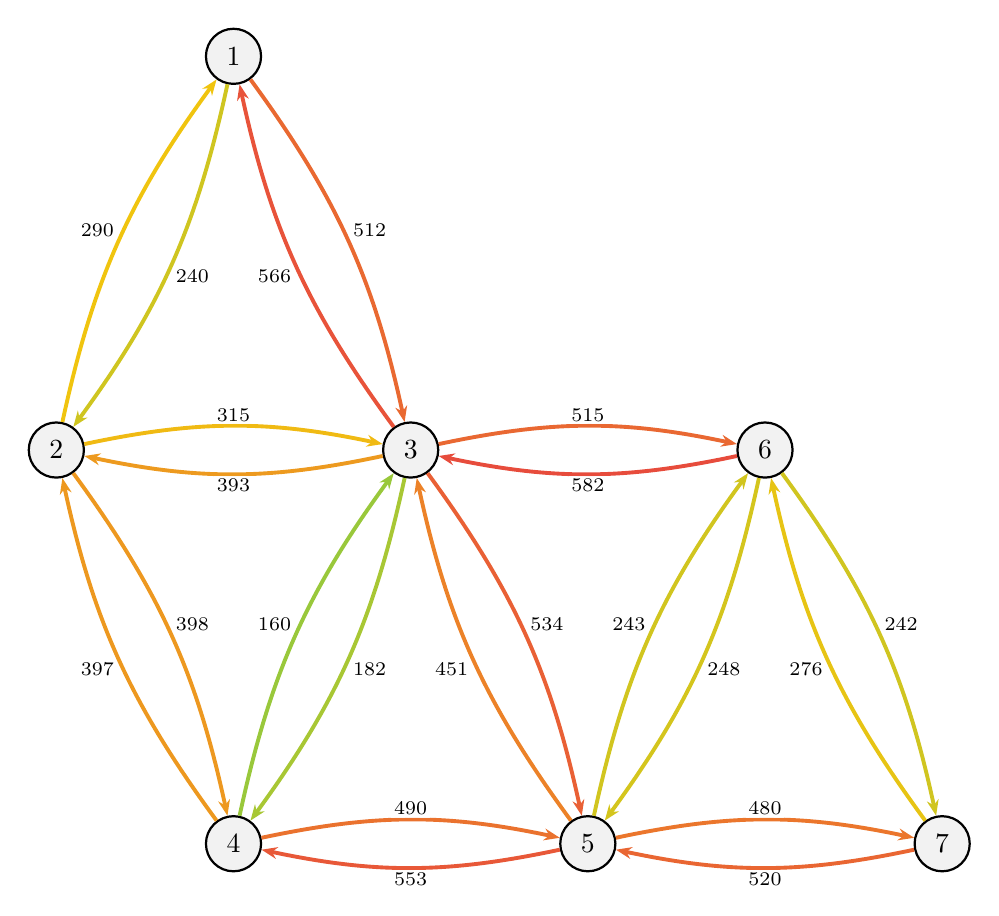
\begin{tikzpicture}[baseline, >={Stealth[length=2mm]},
  netnode/.style={circle, draw, thick, fill=gray!10, minimum size=7mm, inner sep=1pt},
  link/.style={line width=1.4pt},
  linklabel/.style={font=\scriptsize, inner sep=1pt, fill=white, fill opacity=0.85, text opacity=1}]
\node[netnode] (S1) at (2.250,10.000) {1};
\node[netnode] (S2) at (0.000,5.000) {2};
\node[netnode] (S3) at (4.500,5.000) {3};
\node[netnode] (S4) at (2.250,0.000) {4};
\node[netnode] (S5) at (6.750,0.000) {5};
\node[netnode] (S6) at (9.000,5.000) {6};
\node[netnode] (S7) at (11.250,0.000) {7};
\draw[link, ->, draw={rgb,255:red,207;green,197;blue,32}] (S1) to[bend left=12] node[linklabel, auto] {240} (S2);
\draw[link, ->, draw={rgb,255:red,233;green,105;blue,49}] (S1) to[bend left=12] node[linklabel, auto] {512} (S3);
\draw[link, ->, draw={rgb,255:red,240;green,196;blue,15}] (S2) to[bend left=12] node[linklabel, auto] {290} (S1);
\draw[link, ->, draw={rgb,255:red,240;green,186;blue,19}] (S2) to[bend left=12] node[linklabel, auto] {315} (S3);
\draw[link, ->, draw={rgb,255:red,237;green,152;blue,32}] (S2) to[bend left=12] node[linklabel, auto] {398} (S4);
\draw[link, ->, draw={rgb,255:red,232;green,83;blue,58}] (S3) to[bend left=12] node[linklabel, auto] {566} (S1);
\draw[link, ->, draw={rgb,255:red,237;green,154;blue,31}] (S3) to[bend left=12] node[linklabel, auto] {393} (S2);
\draw[link, ->, draw={rgb,255:red,168;green,199;blue,52}] (S3) to[bend left=12] node[linklabel, auto] {182} (S4);
\draw[link, ->, draw={rgb,255:red,233;green,96;blue,53}] (S3) to[bend left=12] node[linklabel, auto] {534} (S5);
\draw[link, ->, draw={rgb,255:red,233;green,104;blue,50}] (S3) to[bend left=12] node[linklabel, auto] {515} (S6);
\draw[link, ->, draw={rgb,255:red,237;green,152;blue,31}] (S4) to[bend left=12] node[linklabel, auto] {397} (S2);
\draw[link, ->, draw={rgb,255:red,153;green,200;blue,59}] (S4) to[bend left=12] node[linklabel, auto] {160} (S3);
\draw[link, ->, draw={rgb,255:red,234;green,114;blue,46}] (S4) to[bend left=12] node[linklabel, auto] {490} (S5);
\draw[link, ->, draw={rgb,255:red,236;green,130;blue,40}] (S5) to[bend left=12] node[linklabel, auto] {451} (S3);
\draw[link, ->, draw={rgb,255:red,232;green,88;blue,56}] (S5) to[bend left=12] node[linklabel, auto] {553} (S4);
\draw[link, ->, draw={rgb,255:red,209;green,197;blue,31}] (S5) to[bend left=12] node[linklabel, auto] {243} (S6);
\draw[link, ->, draw={rgb,255:red,235;green,118;blue,44}] (S5) to[bend left=12] node[linklabel, auto] {480} (S7);
\draw[link, ->, draw={rgb,255:red,231;green,76;blue,60}] (S6) to[bend left=12] node[linklabel, auto] {582} (S3);
\draw[link, ->, draw={rgb,255:red,212;green,197;blue,29}] (S6) to[bend left=12] node[linklabel, auto] {248} (S5);
\draw[link, ->, draw={rgb,255:red,208;green,197;blue,32}] (S6) to[bend left=12] node[linklabel, auto] {242} (S7);
\draw[link, ->, draw={rgb,255:red,233;green,102;blue,50}] (S7) to[bend left=12] node[linklabel, auto] {520} (S5);
\draw[link, ->, draw={rgb,255:red,231;green,196;blue,20}] (S7) to[bend left=12] node[linklabel, auto] {276} (S6);
\end{tikzpicture}
\end{adjustbox}\end{center}
\begin{center}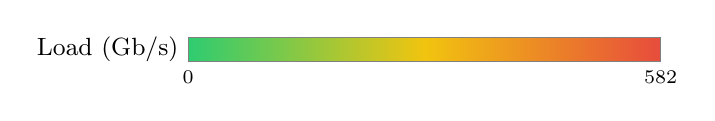
\begin{tikzpicture}
\definecolor{scalelow}{RGB}{46,204,113}\definecolor{scalemid}{RGB}{241,196,15}\definecolor{scalehigh}{RGB}{231,76,60}
\shade[left color=scalelow, right color=scalemid] (0,0) rectangle (3,0.3);
\shade[left color=scalemid, right color=scalehigh] (3,0) rectangle (6,0.3);
\draw[gray] (0,0) rectangle (6,0.3);
\node[below, font=\scriptsize] at (0,0) {0};
\node[below, font=\scriptsize] at (6,0) {582};
\node[left, font=\small] at (0,0.15) {Load (Gb/s)};
\end{tikzpicture}\end{center}
\section*{Link Load Distribution}

\begin{center}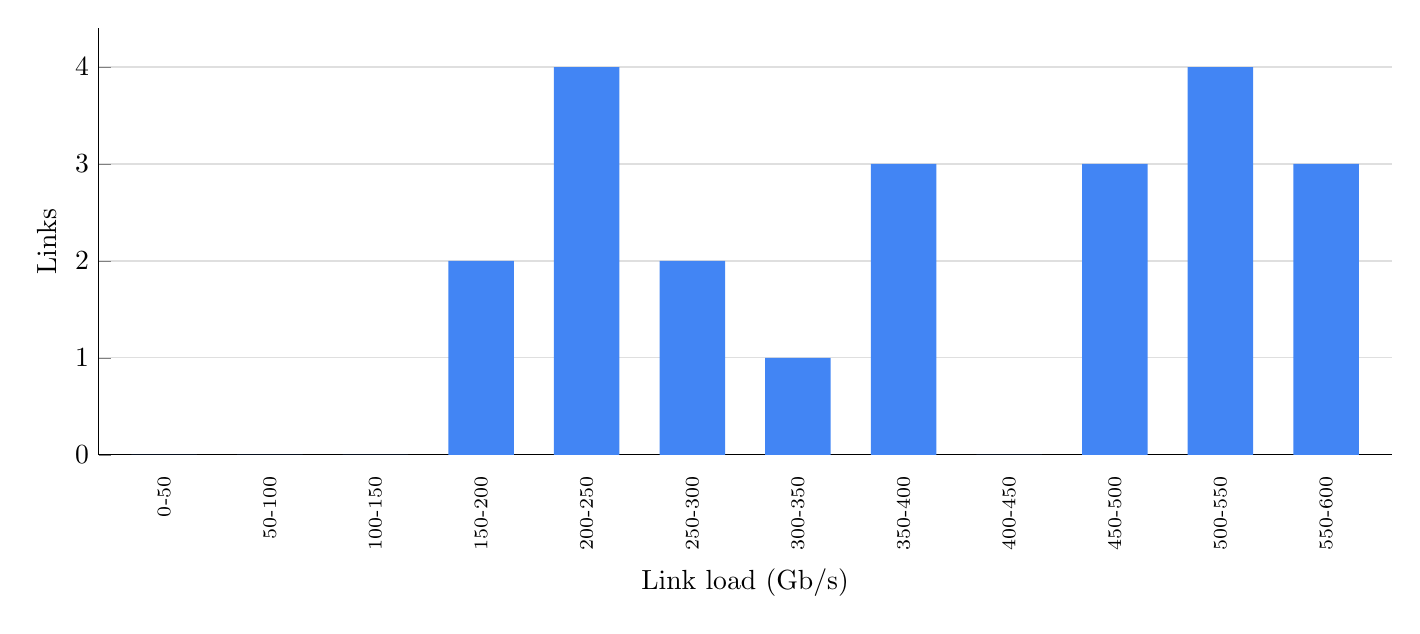
\begin{tikzpicture}
\begin{axis}[
  ybar, bar width=0.831cm, width=18.000cm, height=7cm,
  ymin=0, ymajorgrids, grid style={gray!25}, axis lines*=left,
  enlarge x limits={abs=0.831cm}, xtick=data, major x tick style={draw=none},
  x tick label style={rotate=90, font=\scriptsize, /pgf/number format/1000 sep=},
  legend style={at={(0.5,-0.3)}, anchor=north, legend columns=-1, draw=none},
  ylabel={Links},
  xlabel={Link load (Gb/s)},
  symbolic x coords={0-50,50-100,100-150,150-200,200-250,250-300,300-350,350-400,400-450,450-500,500-550,550-600}]
\addplot[fill={rgb,255:red,66;green,133;blue,244}, draw=none] coordinates {(0-50,0.000) (50-100,0.000) (100-150,0.000) (150-200,2.000) (200-250,4.000) (250-300,2.000) (300-350,1.000) (350-400,3.000) (400-450,0.000) (450-500,3.000) (500-550,4.000) (550-600,3.000) };
\end{axis}
\end{tikzpicture}\end{center}
\clearpage
\section*{Spectrum Occupancy}
\begin{center}\begin{adjustbox}{max width=\linewidth}
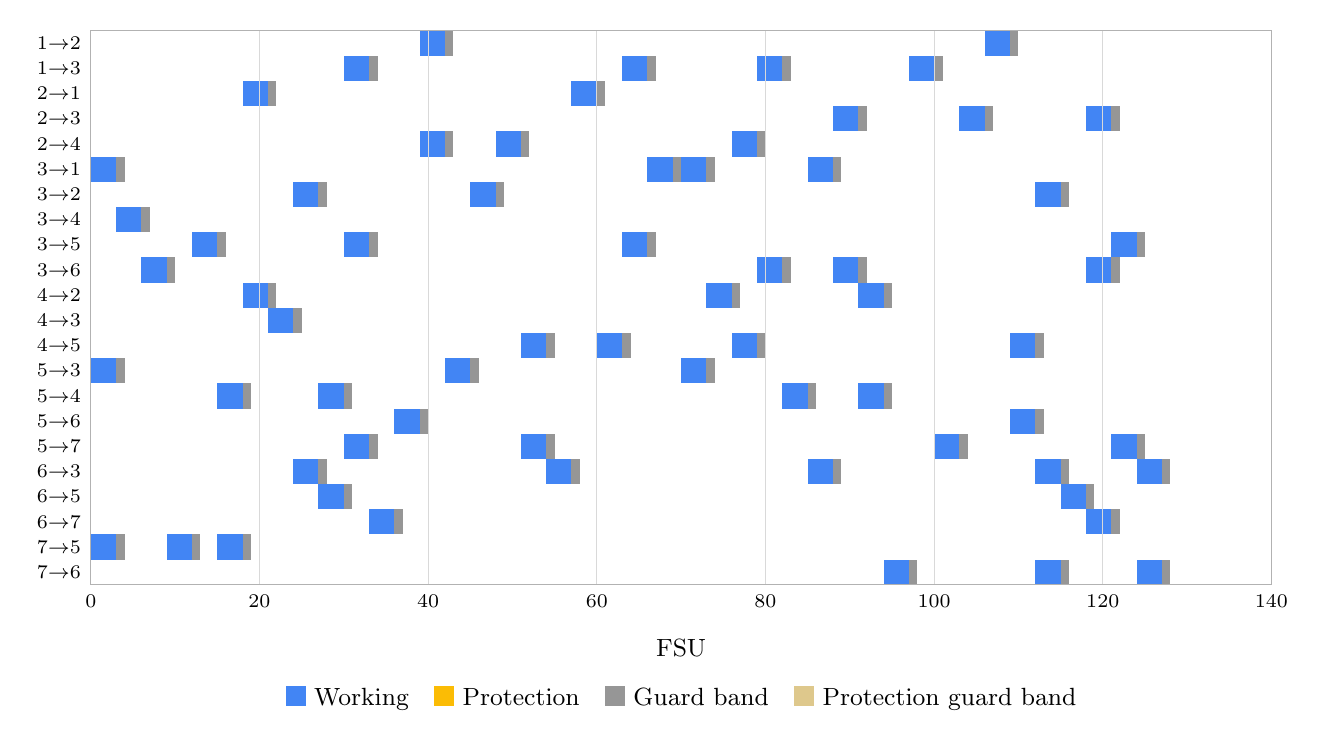
\begin{tikzpicture}[x=0.1071cm, y=-0.32cm]
\fill[fill={rgb,255:red,66;green,133;blue,244}] (39,0) rectangle (42,1);
\fill[fill={rgb,255:red,150;green,150;blue,150}] (42,0) rectangle (43,1);
\fill[fill={rgb,255:red,66;green,133;blue,244}] (106,0) rectangle (109,1);
\fill[fill={rgb,255:red,150;green,150;blue,150}] (109,0) rectangle (110,1);
\node[left, font=\scriptsize] at (0,0.5) {1\(\to\)2};
\fill[fill={rgb,255:red,66;green,133;blue,244}] (30,1) rectangle (33,2);
\fill[fill={rgb,255:red,150;green,150;blue,150}] (33,1) rectangle (34,2);
\fill[fill={rgb,255:red,66;green,133;blue,244}] (63,1) rectangle (66,2);
\fill[fill={rgb,255:red,150;green,150;blue,150}] (66,1) rectangle (67,2);
\fill[fill={rgb,255:red,66;green,133;blue,244}] (79,1) rectangle (82,2);
\fill[fill={rgb,255:red,150;green,150;blue,150}] (82,1) rectangle (83,2);
\fill[fill={rgb,255:red,66;green,133;blue,244}] (97,1) rectangle (100,2);
\fill[fill={rgb,255:red,150;green,150;blue,150}] (100,1) rectangle (101,2);
\node[left, font=\scriptsize] at (0,1.5) {1\(\to\)3};
\fill[fill={rgb,255:red,66;green,133;blue,244}] (18,2) rectangle (21,3);
\fill[fill={rgb,255:red,150;green,150;blue,150}] (21,2) rectangle (22,3);
\fill[fill={rgb,255:red,66;green,133;blue,244}] (57,2) rectangle (60,3);
\fill[fill={rgb,255:red,150;green,150;blue,150}] (60,2) rectangle (61,3);
\node[left, font=\scriptsize] at (0,2.5) {2\(\to\)1};
\fill[fill={rgb,255:red,66;green,133;blue,244}] (88,3) rectangle (91,4);
\fill[fill={rgb,255:red,150;green,150;blue,150}] (91,3) rectangle (92,4);
\fill[fill={rgb,255:red,66;green,133;blue,244}] (103,3) rectangle (106,4);
\fill[fill={rgb,255:red,150;green,150;blue,150}] (106,3) rectangle (107,4);
\fill[fill={rgb,255:red,66;green,133;blue,244}] (118,3) rectangle (121,4);
\fill[fill={rgb,255:red,150;green,150;blue,150}] (121,3) rectangle (122,4);
\node[left, font=\scriptsize] at (0,3.5) {2\(\to\)3};
\fill[fill={rgb,255:red,66;green,133;blue,244}] (39,4) rectangle (42,5);
\fill[fill={rgb,255:red,150;green,150;blue,150}] (42,4) rectangle (43,5);
\fill[fill={rgb,255:red,66;green,133;blue,244}] (48,4) rectangle (51,5);
\fill[fill={rgb,255:red,150;green,150;blue,150}] (51,4) rectangle (52,5);
\fill[fill={rgb,255:red,66;green,133;blue,244}] (76,4) rectangle (79,5);
\fill[fill={rgb,255:red,150;green,150;blue,150}] (79,4) rectangle (80,5);
\node[left, font=\scriptsize] at (0,4.5) {2\(\to\)4};
\fill[fill={rgb,255:red,66;green,133;blue,244}] (0,5) rectangle (3,6);
\fill[fill={rgb,255:red,150;green,150;blue,150}] (3,5) rectangle (4,6);
\fill[fill={rgb,255:red,66;green,133;blue,244}] (66,5) rectangle (69,6);
\fill[fill={rgb,255:red,150;green,150;blue,150}] (69,5) rectangle (70,6);
\fill[fill={rgb,255:red,66;green,133;blue,244}] (70,5) rectangle (73,6);
\fill[fill={rgb,255:red,150;green,150;blue,150}] (73,5) rectangle (74,6);
\fill[fill={rgb,255:red,66;green,133;blue,244}] (85,5) rectangle (88,6);
\fill[fill={rgb,255:red,150;green,150;blue,150}] (88,5) rectangle (89,6);
\node[left, font=\scriptsize] at (0,5.5) {3\(\to\)1};
\fill[fill={rgb,255:red,66;green,133;blue,244}] (24,6) rectangle (27,7);
\fill[fill={rgb,255:red,150;green,150;blue,150}] (27,6) rectangle (28,7);
\fill[fill={rgb,255:red,66;green,133;blue,244}] (45,6) rectangle (48,7);
\fill[fill={rgb,255:red,150;green,150;blue,150}] (48,6) rectangle (49,7);
\fill[fill={rgb,255:red,66;green,133;blue,244}] (112,6) rectangle (115,7);
\fill[fill={rgb,255:red,150;green,150;blue,150}] (115,6) rectangle (116,7);
\node[left, font=\scriptsize] at (0,6.5) {3\(\to\)2};
\fill[fill={rgb,255:red,66;green,133;blue,244}] (3,7) rectangle (6,8);
\fill[fill={rgb,255:red,150;green,150;blue,150}] (6,7) rectangle (7,8);
\node[left, font=\scriptsize] at (0,7.5) {3\(\to\)4};
\fill[fill={rgb,255:red,66;green,133;blue,244}] (12,8) rectangle (15,9);
\fill[fill={rgb,255:red,150;green,150;blue,150}] (15,8) rectangle (16,9);
\fill[fill={rgb,255:red,66;green,133;blue,244}] (30,8) rectangle (33,9);
\fill[fill={rgb,255:red,150;green,150;blue,150}] (33,8) rectangle (34,9);
\fill[fill={rgb,255:red,66;green,133;blue,244}] (63,8) rectangle (66,9);
\fill[fill={rgb,255:red,150;green,150;blue,150}] (66,8) rectangle (67,9);
\fill[fill={rgb,255:red,66;green,133;blue,244}] (121,8) rectangle (124,9);
\fill[fill={rgb,255:red,150;green,150;blue,150}] (124,8) rectangle (125,9);
\node[left, font=\scriptsize] at (0,8.5) {3\(\to\)5};
\fill[fill={rgb,255:red,66;green,133;blue,244}] (6,9) rectangle (9,10);
\fill[fill={rgb,255:red,150;green,150;blue,150}] (9,9) rectangle (10,10);
\fill[fill={rgb,255:red,66;green,133;blue,244}] (79,9) rectangle (82,10);
\fill[fill={rgb,255:red,150;green,150;blue,150}] (82,9) rectangle (83,10);
\fill[fill={rgb,255:red,66;green,133;blue,244}] (88,9) rectangle (91,10);
\fill[fill={rgb,255:red,150;green,150;blue,150}] (91,9) rectangle (92,10);
\fill[fill={rgb,255:red,66;green,133;blue,244}] (118,9) rectangle (121,10);
\fill[fill={rgb,255:red,150;green,150;blue,150}] (121,9) rectangle (122,10);
\node[left, font=\scriptsize] at (0,9.5) {3\(\to\)6};
\fill[fill={rgb,255:red,66;green,133;blue,244}] (18,10) rectangle (21,11);
\fill[fill={rgb,255:red,150;green,150;blue,150}] (21,10) rectangle (22,11);
\fill[fill={rgb,255:red,66;green,133;blue,244}] (73,10) rectangle (76,11);
\fill[fill={rgb,255:red,150;green,150;blue,150}] (76,10) rectangle (77,11);
\fill[fill={rgb,255:red,66;green,133;blue,244}] (91,10) rectangle (94,11);
\fill[fill={rgb,255:red,150;green,150;blue,150}] (94,10) rectangle (95,11);
\node[left, font=\scriptsize] at (0,10.5) {4\(\to\)2};
\fill[fill={rgb,255:red,66;green,133;blue,244}] (21,11) rectangle (24,12);
\fill[fill={rgb,255:red,150;green,150;blue,150}] (24,11) rectangle (25,12);
\node[left, font=\scriptsize] at (0,11.5) {4\(\to\)3};
\fill[fill={rgb,255:red,66;green,133;blue,244}] (51,12) rectangle (54,13);
\fill[fill={rgb,255:red,150;green,150;blue,150}] (54,12) rectangle (55,13);
\fill[fill={rgb,255:red,66;green,133;blue,244}] (60,12) rectangle (63,13);
\fill[fill={rgb,255:red,150;green,150;blue,150}] (63,12) rectangle (64,13);
\fill[fill={rgb,255:red,66;green,133;blue,244}] (76,12) rectangle (79,13);
\fill[fill={rgb,255:red,150;green,150;blue,150}] (79,12) rectangle (80,13);
\fill[fill={rgb,255:red,66;green,133;blue,244}] (109,12) rectangle (112,13);
\fill[fill={rgb,255:red,150;green,150;blue,150}] (112,12) rectangle (113,13);
\node[left, font=\scriptsize] at (0,12.5) {4\(\to\)5};
\fill[fill={rgb,255:red,66;green,133;blue,244}] (0,13) rectangle (3,14);
\fill[fill={rgb,255:red,150;green,150;blue,150}] (3,13) rectangle (4,14);
\fill[fill={rgb,255:red,66;green,133;blue,244}] (42,13) rectangle (45,14);
\fill[fill={rgb,255:red,150;green,150;blue,150}] (45,13) rectangle (46,14);
\fill[fill={rgb,255:red,66;green,133;blue,244}] (70,13) rectangle (73,14);
\fill[fill={rgb,255:red,150;green,150;blue,150}] (73,13) rectangle (74,14);
\node[left, font=\scriptsize] at (0,13.5) {5\(\to\)3};
\fill[fill={rgb,255:red,66;green,133;blue,244}] (15,14) rectangle (18,15);
\fill[fill={rgb,255:red,150;green,150;blue,150}] (18,14) rectangle (19,15);
\fill[fill={rgb,255:red,66;green,133;blue,244}] (27,14) rectangle (30,15);
\fill[fill={rgb,255:red,150;green,150;blue,150}] (30,14) rectangle (31,15);
\fill[fill={rgb,255:red,66;green,133;blue,244}] (82,14) rectangle (85,15);
\fill[fill={rgb,255:red,150;green,150;blue,150}] (85,14) rectangle (86,15);
\fill[fill={rgb,255:red,66;green,133;blue,244}] (91,14) rectangle (94,15);
\fill[fill={rgb,255:red,150;green,150;blue,150}] (94,14) rectangle (95,15);
\node[left, font=\scriptsize] at (0,14.5) {5\(\to\)4};
\fill[fill={rgb,255:red,66;green,133;blue,244}] (36,15) rectangle (39,16);
\fill[fill={rgb,255:red,150;green,150;blue,150}] (39,15) rectangle (40,16);
\fill[fill={rgb,255:red,66;green,133;blue,244}] (109,15) rectangle (112,16);
\fill[fill={rgb,255:red,150;green,150;blue,150}] (112,15) rectangle (113,16);
\node[left, font=\scriptsize] at (0,15.5) {5\(\to\)6};
\fill[fill={rgb,255:red,66;green,133;blue,244}] (30,16) rectangle (33,17);
\fill[fill={rgb,255:red,150;green,150;blue,150}] (33,16) rectangle (34,17);
\fill[fill={rgb,255:red,66;green,133;blue,244}] (51,16) rectangle (54,17);
\fill[fill={rgb,255:red,150;green,150;blue,150}] (54,16) rectangle (55,17);
\fill[fill={rgb,255:red,66;green,133;blue,244}] (100,16) rectangle (103,17);
\fill[fill={rgb,255:red,150;green,150;blue,150}] (103,16) rectangle (104,17);
\fill[fill={rgb,255:red,66;green,133;blue,244}] (121,16) rectangle (124,17);
\fill[fill={rgb,255:red,150;green,150;blue,150}] (124,16) rectangle (125,17);
\node[left, font=\scriptsize] at (0,16.5) {5\(\to\)7};
\fill[fill={rgb,255:red,66;green,133;blue,244}] (24,17) rectangle (27,18);
\fill[fill={rgb,255:red,150;green,150;blue,150}] (27,17) rectangle (28,18);
\fill[fill={rgb,255:red,66;green,133;blue,244}] (54,17) rectangle (57,18);
\fill[fill={rgb,255:red,150;green,150;blue,150}] (57,17) rectangle (58,18);
\fill[fill={rgb,255:red,66;green,133;blue,244}] (85,17) rectangle (88,18);
\fill[fill={rgb,255:red,150;green,150;blue,150}] (88,17) rectangle (89,18);
\fill[fill={rgb,255:red,66;green,133;blue,244}] (112,17) rectangle (115,18);
\fill[fill={rgb,255:red,150;green,150;blue,150}] (115,17) rectangle (116,18);
\fill[fill={rgb,255:red,66;green,133;blue,244}] (124,17) rectangle (127,18);
\fill[fill={rgb,255:red,150;green,150;blue,150}] (127,17) rectangle (128,18);
\node[left, font=\scriptsize] at (0,17.5) {6\(\to\)3};
\fill[fill={rgb,255:red,66;green,133;blue,244}] (27,18) rectangle (30,19);
\fill[fill={rgb,255:red,150;green,150;blue,150}] (30,18) rectangle (31,19);
\fill[fill={rgb,255:red,66;green,133;blue,244}] (115,18) rectangle (118,19);
\fill[fill={rgb,255:red,150;green,150;blue,150}] (118,18) rectangle (119,19);
\node[left, font=\scriptsize] at (0,18.5) {6\(\to\)5};
\fill[fill={rgb,255:red,66;green,133;blue,244}] (33,19) rectangle (36,20);
\fill[fill={rgb,255:red,150;green,150;blue,150}] (36,19) rectangle (37,20);
\fill[fill={rgb,255:red,66;green,133;blue,244}] (118,19) rectangle (121,20);
\fill[fill={rgb,255:red,150;green,150;blue,150}] (121,19) rectangle (122,20);
\node[left, font=\scriptsize] at (0,19.5) {6\(\to\)7};
\fill[fill={rgb,255:red,66;green,133;blue,244}] (0,20) rectangle (3,21);
\fill[fill={rgb,255:red,150;green,150;blue,150}] (3,20) rectangle (4,21);
\fill[fill={rgb,255:red,66;green,133;blue,244}] (9,20) rectangle (12,21);
\fill[fill={rgb,255:red,150;green,150;blue,150}] (12,20) rectangle (13,21);
\fill[fill={rgb,255:red,66;green,133;blue,244}] (15,20) rectangle (18,21);
\fill[fill={rgb,255:red,150;green,150;blue,150}] (18,20) rectangle (19,21);
\node[left, font=\scriptsize] at (0,20.5) {7\(\to\)5};
\fill[fill={rgb,255:red,66;green,133;blue,244}] (94,21) rectangle (97,22);
\fill[fill={rgb,255:red,150;green,150;blue,150}] (97,21) rectangle (98,22);
\fill[fill={rgb,255:red,66;green,133;blue,244}] (112,21) rectangle (115,22);
\fill[fill={rgb,255:red,150;green,150;blue,150}] (115,21) rectangle (116,22);
\fill[fill={rgb,255:red,66;green,133;blue,244}] (124,21) rectangle (127,22);
\fill[fill={rgb,255:red,150;green,150;blue,150}] (127,21) rectangle (128,22);
\node[left, font=\scriptsize] at (0,21.5) {7\(\to\)6};
\foreach \s in {0,20,...,140} {\draw[gray!30] (\s,0) -- (\s,22); \node[below, font=\scriptsize] at (\s,22) {\s};}
\draw[gray!60] (0,0) rectangle (140,22);
\node[font=\small] at (70.0,24.5) {FSU};
\node[font=\small] at (70.0,26.5) {\textcolor[RGB]{66,133,244}{\rule{2.5mm}{2.5mm}} Working\quad \textcolor[RGB]{251,188,5}{\rule{2.5mm}{2.5mm}} Protection\quad \textcolor[RGB]{150,150,150}{\rule{2.5mm}{2.5mm}} Guard band\quad \textcolor[RGB]{222,200,140}{\rule{2.5mm}{2.5mm}} Protection guard band\quad };
\end{tikzpicture}
\end{adjustbox}\end{center}
\clearpage
\section*{Path Length Distribution}

\begin{center}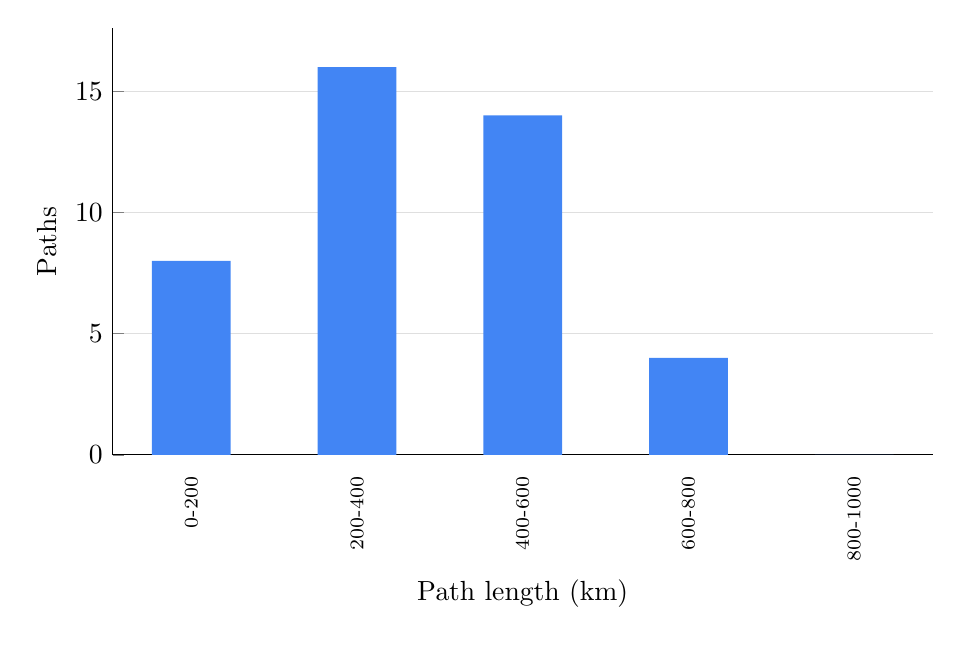
\begin{tikzpicture}
\begin{axis}[
  ybar, bar width=1.000cm, width=12.000cm, height=7cm,
  ymin=0, ymajorgrids, grid style={gray!25}, axis lines*=left,
  enlarge x limits={abs=1.000cm}, xtick=data, major x tick style={draw=none},
  x tick label style={rotate=90, font=\scriptsize, /pgf/number format/1000 sep=},
  legend style={at={(0.5,-0.3)}, anchor=north, legend columns=-1, draw=none},
  ylabel={Paths},
  xlabel={Path length (km)},
  symbolic x coords={0-200,200-400,400-600,600-800,800-1000,1000-1200,1200-1400,1400-1600,1600-1800,1800-2000}]
\addplot[fill={rgb,255:red,66;green,133;blue,244}, draw=none] coordinates {(0-200,8.000) (200-400,16.000) (400-600,14.000) (600-800,4.000) (800-1000,0.000) };
\end{axis}
\end{tikzpicture}\end{center}
\clearpage
\section*{Utilization Entropy}
\begin{center}\begin{adjustbox}{max width=\linewidth}
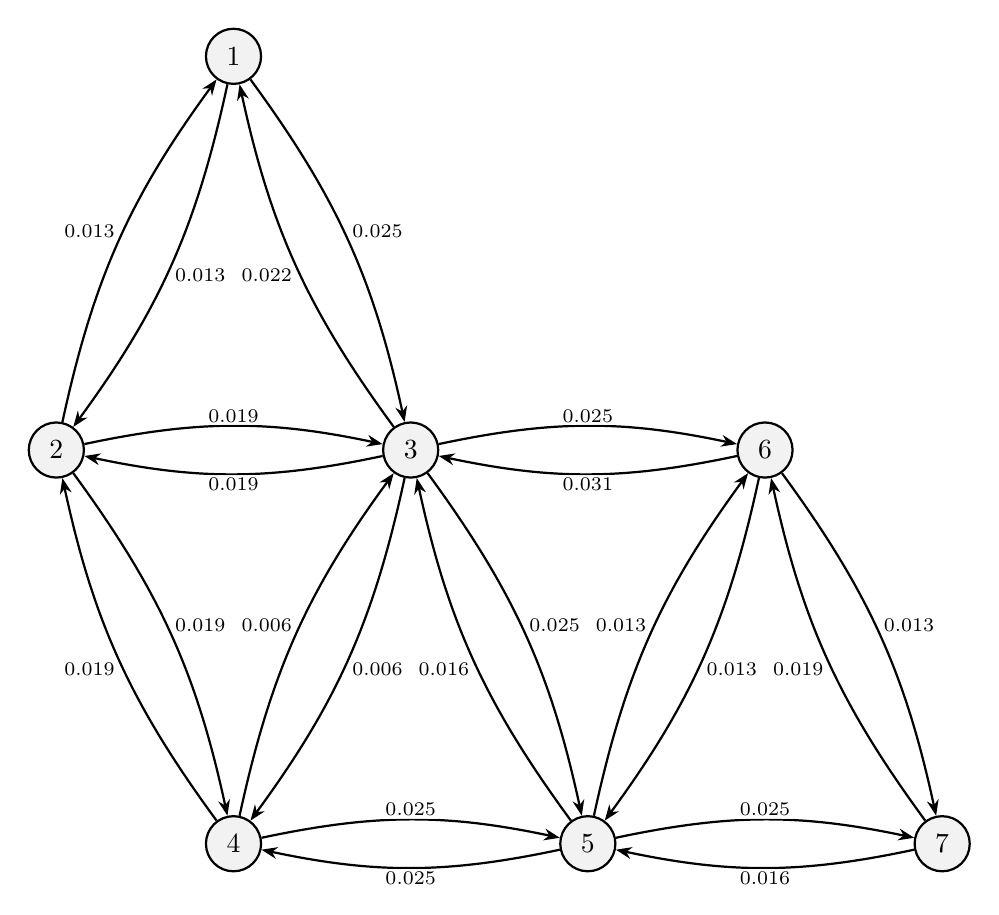
\begin{tikzpicture}[baseline, >={Stealth[length=2mm]},
  netnode/.style={circle, draw, thick, fill=gray!10, minimum size=7mm, inner sep=1pt},
  link/.style={thick},
  linklabel/.style={font=\scriptsize, inner sep=1pt, fill=white, fill opacity=0.85, text opacity=1}]
\node[netnode] (S1) at (2.250,10.000) {1};
\node[netnode] (S2) at (0.000,5.000) {2};
\node[netnode] (S3) at (4.500,5.000) {3};
\node[netnode] (S4) at (2.250,0.000) {4};
\node[netnode] (S5) at (6.750,0.000) {5};
\node[netnode] (S6) at (9.000,5.000) {6};
\node[netnode] (S7) at (11.250,0.000) {7};
\draw[link, ->] (S1) to[bend left=12] node[linklabel, auto] {0.013} (S2);
\draw[link, ->] (S1) to[bend left=12] node[linklabel, auto] {0.025} (S3);
\draw[link, ->] (S2) to[bend left=12] node[linklabel, auto] {0.013} (S1);
\draw[link, ->] (S2) to[bend left=12] node[linklabel, auto] {0.019} (S3);
\draw[link, ->] (S2) to[bend left=12] node[linklabel, auto] {0.019} (S4);
\draw[link, ->] (S3) to[bend left=12] node[linklabel, auto] {0.022} (S1);
\draw[link, ->] (S3) to[bend left=12] node[linklabel, auto] {0.019} (S2);
\draw[link, ->] (S3) to[bend left=12] node[linklabel, auto] {0.006} (S4);
\draw[link, ->] (S3) to[bend left=12] node[linklabel, auto] {0.025} (S5);
\draw[link, ->] (S3) to[bend left=12] node[linklabel, auto] {0.025} (S6);
\draw[link, ->] (S4) to[bend left=12] node[linklabel, auto] {0.019} (S2);
\draw[link, ->] (S4) to[bend left=12] node[linklabel, auto] {0.006} (S3);
\draw[link, ->] (S4) to[bend left=12] node[linklabel, auto] {0.025} (S5);
\draw[link, ->] (S5) to[bend left=12] node[linklabel, auto] {0.016} (S3);
\draw[link, ->] (S5) to[bend left=12] node[linklabel, auto] {0.025} (S4);
\draw[link, ->] (S5) to[bend left=12] node[linklabel, auto] {0.013} (S6);
\draw[link, ->] (S5) to[bend left=12] node[linklabel, auto] {0.025} (S7);
\draw[link, ->] (S6) to[bend left=12] node[linklabel, auto] {0.031} (S3);
\draw[link, ->] (S6) to[bend left=12] node[linklabel, auto] {0.013} (S5);
\draw[link, ->] (S6) to[bend left=12] node[linklabel, auto] {0.013} (S7);
\draw[link, ->] (S7) to[bend left=12] node[linklabel, auto] {0.016} (S5);
\draw[link, ->] (S7) to[bend left=12] node[linklabel, auto] {0.019} (S6);
\end{tikzpicture}
\end{adjustbox}\end{center}

\begin{center}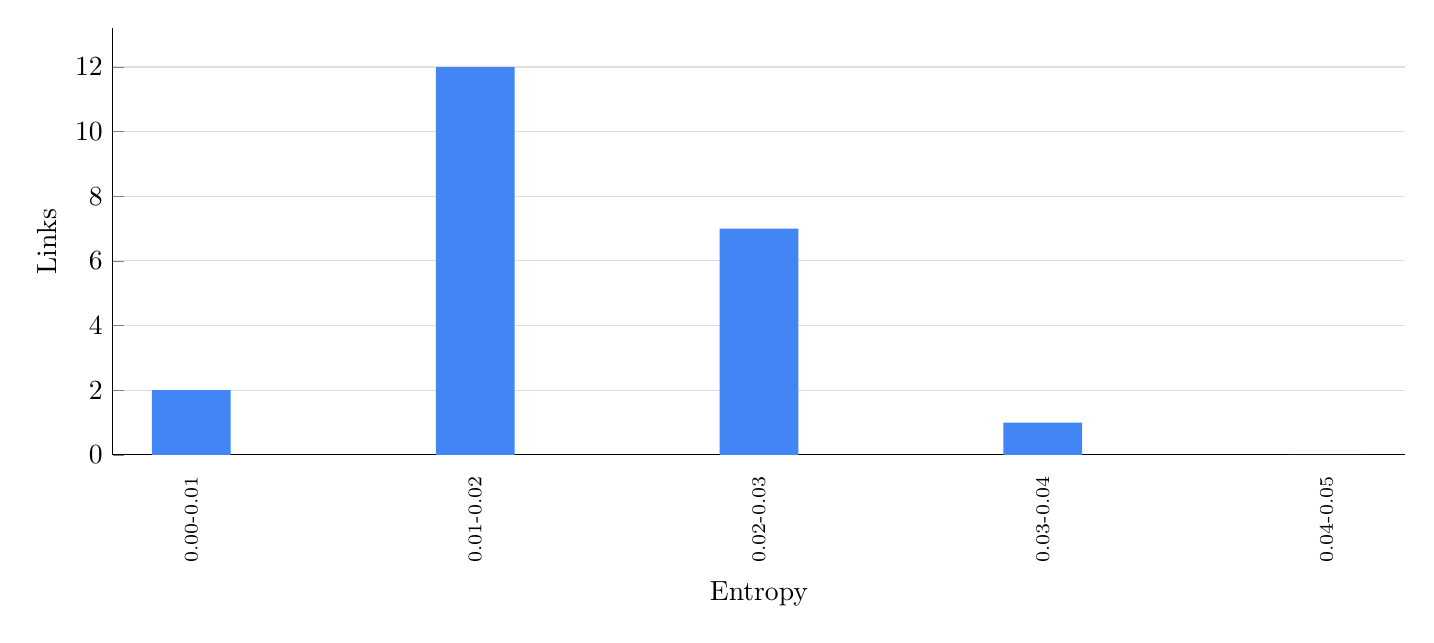
\begin{tikzpicture}
\begin{axis}[
  ybar, bar width=1.000cm, width=18.000cm, height=7cm,
  ymin=0, ymajorgrids, grid style={gray!25}, axis lines*=left,
  enlarge x limits={abs=1.000cm}, xtick=data, major x tick style={draw=none},
  x tick label style={rotate=90, font=\scriptsize, /pgf/number format/1000 sep=},
  legend style={at={(0.5,-0.3)}, anchor=north, legend columns=-1, draw=none},
  ylabel={Links},
  xlabel={Entropy},
  symbolic x coords={0.00-0.01,0.01-0.02,0.02-0.03,0.03-0.04,0.04-0.05,0.05-0.06,0.06-0.07,0.07-0.08,0.08-0.09,0.09-0.10,0.10-0.11,0.11-0.12,0.12-0.13,0.13-0.14,0.14-0.15,0.15-0.16,0.16-0.17,0.17-0.18,0.18-0.19,0.19-0.20,0.20-0.21,0.21-0.22,0.22-0.23,0.23-0.24,0.24-0.25,0.25-0.26,0.26-0.27,0.27-0.28,0.28-0.29,0.29-0.30,0.30-0.31,0.31-0.32,0.32-0.33,0.33-0.34,0.34-0.35,0.35-0.36,0.36-0.37,0.37-0.38,0.38-0.39,0.39-0.40,0.40-0.41,0.41-0.42,0.42-0.43,0.43-0.44,0.44-0.45,0.45-0.46,0.46-0.47,0.47-0.48,0.48-0.49,0.49-0.50,0.50-0.51,0.51-0.52,0.52-0.53,0.53-0.54,0.54-0.55,0.55-0.56,0.56-0.57,0.57-0.58,0.58-0.59,0.59-0.60,0.60-0.61,0.61-0.62,0.62-0.63,0.63-0.64,0.64-0.65,0.65-0.66,0.66-0.67,0.67-0.68,0.68-0.69,0.69-0.70,0.70-0.71,0.71-0.72,0.72-0.73,0.73-0.74,0.74-0.75,0.75-0.76,0.76-0.77,0.77-0.78,0.78-0.79,0.79-0.80,0.80-0.81,0.81-0.82,0.82-0.83,0.83-0.84,0.84-0.85,0.85-0.86,0.86-0.87,0.87-0.88,0.88-0.89,0.89-0.90,0.90-0.91,0.91-0.92,0.92-0.93,0.93-0.94,0.94-0.95,0.95-0.96,0.96-0.97,0.97-0.98,0.98-0.99,0.99-1.00}]
\addplot[fill={rgb,255:red,66;green,133;blue,244}, draw=none] coordinates {(0.00-0.01,2.000) (0.01-0.02,12.000) (0.02-0.03,7.000) (0.03-0.04,1.000) (0.04-0.05,0.000) };
\end{axis}
\end{tikzpicture}\end{center}
\clearpage
\section*{Shannon Entropy}
\begin{center}\begin{adjustbox}{max width=\linewidth}
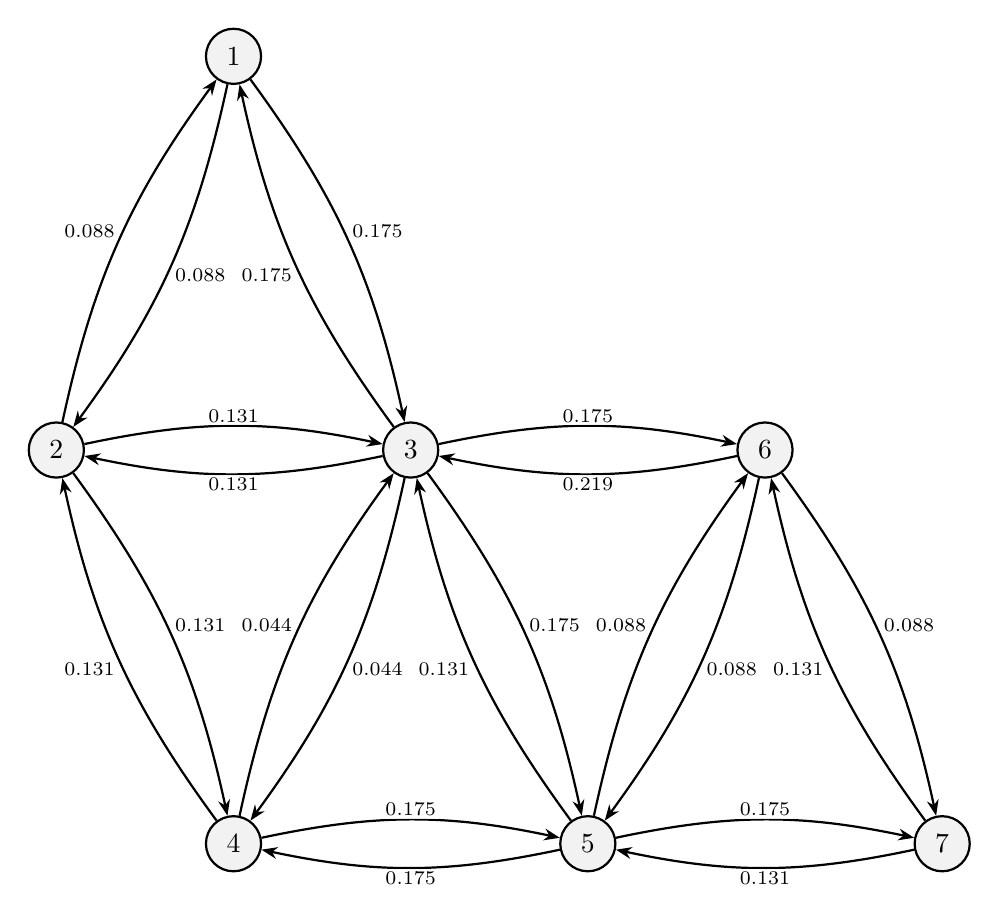
\begin{tikzpicture}[baseline, >={Stealth[length=2mm]},
  netnode/.style={circle, draw, thick, fill=gray!10, minimum size=7mm, inner sep=1pt},
  link/.style={thick},
  linklabel/.style={font=\scriptsize, inner sep=1pt, fill=white, fill opacity=0.85, text opacity=1}]
\node[netnode] (S1) at (2.250,10.000) {1};
\node[netnode] (S2) at (0.000,5.000) {2};
\node[netnode] (S3) at (4.500,5.000) {3};
\node[netnode] (S4) at (2.250,0.000) {4};
\node[netnode] (S5) at (6.750,0.000) {5};
\node[netnode] (S6) at (9.000,5.000) {6};
\node[netnode] (S7) at (11.250,0.000) {7};
\draw[link, ->] (S1) to[bend left=12] node[linklabel, auto] {0.088} (S2);
\draw[link, ->] (S1) to[bend left=12] node[linklabel, auto] {0.175} (S3);
\draw[link, ->] (S2) to[bend left=12] node[linklabel, auto] {0.088} (S1);
\draw[link, ->] (S2) to[bend left=12] node[linklabel, auto] {0.131} (S3);
\draw[link, ->] (S2) to[bend left=12] node[linklabel, auto] {0.131} (S4);
\draw[link, ->] (S3) to[bend left=12] node[linklabel, auto] {0.175} (S1);
\draw[link, ->] (S3) to[bend left=12] node[linklabel, auto] {0.131} (S2);
\draw[link, ->] (S3) to[bend left=12] node[linklabel, auto] {0.044} (S4);
\draw[link, ->] (S3) to[bend left=12] node[linklabel, auto] {0.175} (S5);
\draw[link, ->] (S3) to[bend left=12] node[linklabel, auto] {0.175} (S6);
\draw[link, ->] (S4) to[bend left=12] node[linklabel, auto] {0.131} (S2);
\draw[link, ->] (S4) to[bend left=12] node[linklabel, auto] {0.044} (S3);
\draw[link, ->] (S4) to[bend left=12] node[linklabel, auto] {0.175} (S5);
\draw[link, ->] (S5) to[bend left=12] node[linklabel, auto] {0.131} (S3);
\draw[link, ->] (S5) to[bend left=12] node[linklabel, auto] {0.175} (S4);
\draw[link, ->] (S5) to[bend left=12] node[linklabel, auto] {0.088} (S6);
\draw[link, ->] (S5) to[bend left=12] node[linklabel, auto] {0.175} (S7);
\draw[link, ->] (S6) to[bend left=12] node[linklabel, auto] {0.219} (S3);
\draw[link, ->] (S6) to[bend left=12] node[linklabel, auto] {0.088} (S5);
\draw[link, ->] (S6) to[bend left=12] node[linklabel, auto] {0.088} (S7);
\draw[link, ->] (S7) to[bend left=12] node[linklabel, auto] {0.131} (S5);
\draw[link, ->] (S7) to[bend left=12] node[linklabel, auto] {0.131} (S6);
\end{tikzpicture}
\end{adjustbox}\end{center}

\begin{center}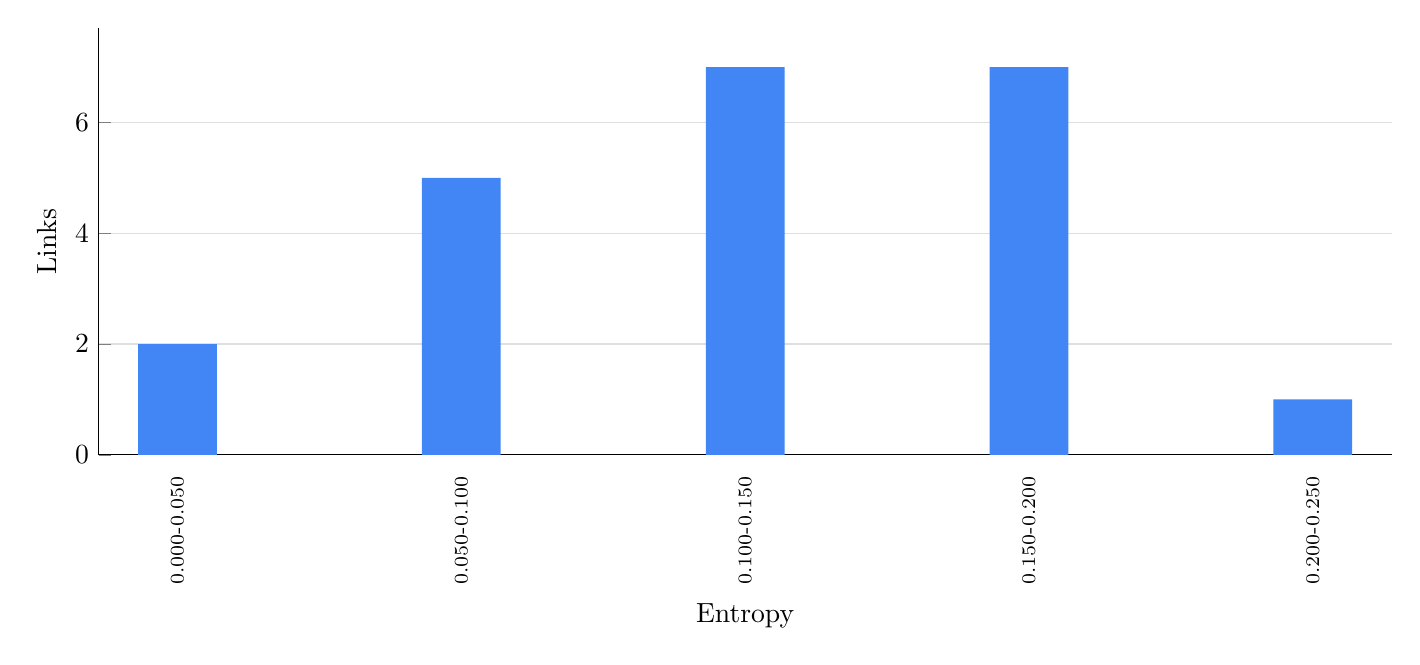
\begin{tikzpicture}
\begin{axis}[
  ybar, bar width=1.000cm, width=18.000cm, height=7cm,
  ymin=0, ymajorgrids, grid style={gray!25}, axis lines*=left,
  enlarge x limits={abs=1.000cm}, xtick=data, major x tick style={draw=none},
  x tick label style={rotate=90, font=\scriptsize, /pgf/number format/1000 sep=},
  legend style={at={(0.5,-0.3)}, anchor=north, legend columns=-1, draw=none},
  ylabel={Links},
  xlabel={Entropy},
  symbolic x coords={0.000-0.050,0.050-0.100,0.100-0.150,0.150-0.200,0.200-0.250,0.250-0.300,0.300-0.350,0.350-0.400,0.400-0.450,0.450-0.500,0.500-0.550,0.550-0.600,0.600-0.650,0.650-0.700,0.700-0.750,0.750-0.800,0.800-0.850,0.850-0.900,0.900-0.950,0.950-1.000}]
\addplot[fill={rgb,255:red,66;green,133;blue,244}, draw=none] coordinates {(0.000-0.050,2.000) (0.050-0.100,5.000) (0.100-0.150,7.000) (0.150-0.200,7.000) (0.200-0.250,1.000) };
\end{axis}
\end{tikzpicture}\end{center}

\end{document}
